\section{Theoretische Grundlagen}
\label{sec:theorie}

\subsection{Aufbau eines Lasers}

Ein Laser besteht aus drei elementaren Komponenten: der \textit{Energiepumpe}, dem \textit{verstärkenden Medium} und dem \textit{Resonator}. \\
Die Energiepumpe pumpt die Atome im Lasermedium z.B. mithilfe von Photonen auf höhere Energieniveaus. 
Bei genügender Pumpleistung wird die Besetzungsdichte $N_k$ auf einem Energieniveau $E_k$ höher als die Besetzungsdichte $N_i$ auf einem niedrigeren Energieniveau $E_i$.
Dieser Zustand wird Inversion genannt \cite{dem01}.
So kann das Licht beim Durchgang durch das aktive Medium verstärkt werden. \\

Der Resonator ist aus zwei Spiegeln aufgebaut, die das Licht reflektieren und erneut durch das verstärkende Medium schicken.
Einer dieser Spiegel ist totalreflektierend, der andere wirft nur einen Teil des Lichts zurück, sodass das restliche Licht aus dem Laser entweichen kann.
Die Stabilität des Resonators wird durch den Stabilitätsfaktor
\begin{equation}
    g_i := 1 - \frac{L}{r_i} 
\end{equation}
beschrieben, wobei $L$ die Resonatorlänge und $r_i$ den Krümmungsradius des betrachteten Spiegels darstellt.
Der Resonator gilt als stabil, solange $0 < g_1 g_2 \leq 1$ gilt \cite{dem01}.

\subsection{Das Zwei-Niveau-System}
\label{subsec:2nivsys}

Auch wenn, wie im Folgenden gezeigt, Zwei-Niveau-Systeme für Laser ungeeignet sind, ist die Betrachtung dieser dennoch hilfreich. \\
Im Zwei-Niveau-System existieren zwei Energiezustände, $E_0$ und $E_1$, mit $\Delta E = E_0 - E_1 < 0$. \\
Ein eintreffendes, stimulierendes Photon, das mindestens die Energie $\Delta E$ besitzt, kann das System, das sich in $E_1$ befindet, auf das höhere Energieniveau anheben und wird dabei absorbiert.
Das System kann nun auf zwei Arten in den Grundzustand zurückkehren: durch \textit{spontane Emission} eines Photons, oder \textit{induzierte Emission}, die durch ein externes Photon der passenden Energie ausgelöst wird.
Das so stimulierte Photon besitzt die gleiche Energie, Phase und Polarisation wie das stimulierende Photon. \\

Eine schematische Darstellung dieser Prozesse findet sich in \autoref{fig:abemiss}.

\begin{figure}[H]
    \centering
    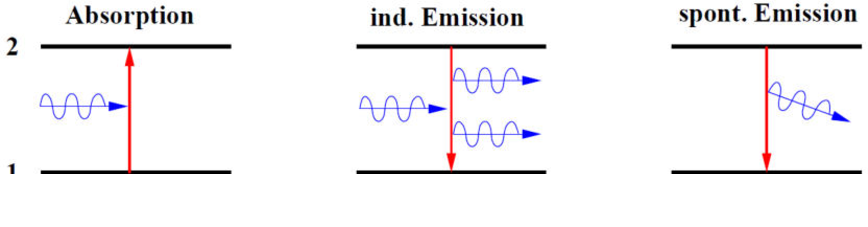
\includegraphics{figures/Absorption_Emission.pdf}
    \caption{Schematische Darstellung der Absorption, induzierten und spontanen Emission in einem Zwei-Niveau-System.}
    \label{fig:abemiss}
\end{figure}

Mit der spektralen Strahldichte $\rho$ ergeben sich die zeitlichen Änderungen der Atome $N_i$ im Energiezustand $E_i$ nach \cite{dem01} zu

\begin{align}
    \frac{\dif N_1}{\dif t} &= - N_1 \rho B_{12} + N_2 \rho B_{21} + N_2 A_{21} \label{eq:dN1} \,, \\
    \frac{\dif N_2}{\dif t} &= + N_1 \rho B_{12} - N_2 \rho B_{21} - N_2 A_{21} \label{eq:dN2} \,, 
\end{align}
wobei $A$ die spontane Emission im Resonator, $B_{21}$ die induzierte Emission und $B_{12}$ die Absorption als nicht näher bestimmte Proportionalitätskonstanten beschreiben. \\
Wie zu erkennen ist gilt $\frac{\dif N_1}{\dif t} = -\frac{\dif N_2}{\dif t}$, mit $\Delta N = N_1 - N_2$, $B_{12} = B_{21}$ und $A_{21} = A$ folgt also
\begin{equation}
    \frac{\dif \Delta N}{\dif t} = - 2 B \rho \Delta N + A N - A \Delta N \,.
    \label{eq:deltaN}
\end{equation}
Dabei ist $N = N_1 + N_2$.
Den obigen Gleichungen nach kann also keine Besetzungsinversion erzielt werden, die Anzahl der Zustände auf $E_1$ kann niemals größer als die Anzahl der Zustände auf $E_0$ sein.
Für einen Laser wird also ein System mit höheren Energieniveaus benötigt.

\subsection{Der Helium-Neon-Laser}

Das HeNe-Gasgemisch im Inneren des HeNe-Lasers kann durch ein Vier-Niveau-System beschrieben werden.
Dabei gilt die Ordnung $E_0 < E_1 < E_2 < E_3$. Wichtig ist, dass Übergänge von $E_3$ nach $E_2$ sowie $E_1$ nach $E_0$ deutlich schneller als Übergänge von $E_2$ nach $E_1$ stattfinden.
Dass die beschriebenen schnellen, metastabilen Übergänge auf näherungsweise vernachlässigbaren Zeitskalen stattfinden, lässt eine zu \autoref{subsec:2nivsys} analoge Betrachtung mit
$N \approx N_0 + N_2$ und $\Delta N \approx - N_2$ zu, sodass sich die Änderungsraten zu
\begin{align*}
    \frac{\dif N_1}{\dif t} &\approx 0 \\
    \frac{\dif N_2}{\dif t} &= N_0 \rho B_{12} - N_2 A_{21}
\end{align*}
ergeben. \\
Hier ergibt sich immer eine negative Besetzung. \\

Der konkrete Ablauf von Anregung und Emission ist in \autoref{fig:HeNeUebergaenge} näher dargestellt.

\begin{figure}[H]
    \centering
    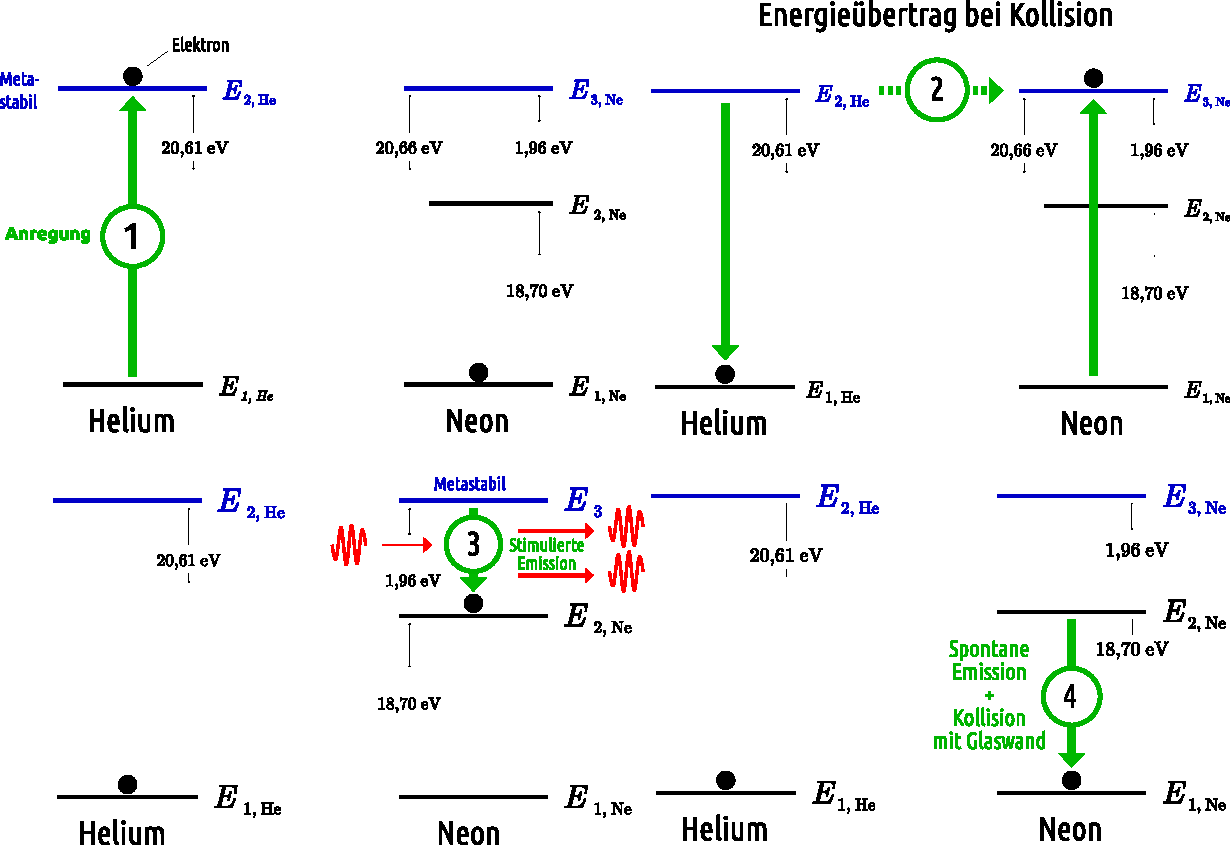
\includegraphics[width=\textwidth]{figures/HeNe-LaserÜbergänge.pdf}
    \caption{Schema der im HeNe-Gemisch des Lasers stattfindenden Übergänge \cite{leifi}. In Schritt 1 wird das Helium von seinem Grundzustand auf den höheren Zustand $E_{2,\text{He}}$ angeregt und gibt bei einem Stoß
    mit einem Neonatom seine Energie an dieses ab (Schritt 2). Bei Stimulierter Emission durch ein äußeres Photon fällt das Neon auf einen niedrigeren Energiezustand zurück und emittiert dabei Photonen, darunter unter
    anderem die bekannte $633 \,\unit{\nano\meter}$-Linie (Schritt 3). Durch Kollision mit der Gefäßwand gibt das Neon dann seine restliche Energie ab und fällt in den Grundzustand zurück.}
    \label{fig:HeNeUebergaenge}
\end{figure}

